%%%%%%%%%%%%%%%%%%%%%%%%%%%%%%%%%%%%%%%%%%%%%%%%%%%%%%%%%%%%%%%%%%%%%%
%%                     absolute stimulation
%%%%%%%%%%%%%%%%%%%%%%%%%%%%%%%%%%%%%%%%%%%%%%%%%%%%%%%%%%%%%%%%%%%%%%
%\color{red}

\subsubsection{Glyph: \glyph{Absolute stimulation}}\label{sec:absoluteStimulation}

An absolute stimulation always triggers the existence of a target relationship. 

\begin{glyphDescription}
 \glyphSboTerm SBO:0000411 ! absolute stimulation
 \glyphOrigin Any \glyph{entity node} (\sect{ENs}).
 \glyphTarget Any \glyph{relationship} (\sect{relationships}).
 \glyphEndPoint The target extremity of a \glyph{absolute stimulation} carries a double empty arrowhead (to remind that it is a \glyph{stimulation}).
 \glyphAux A \glyph{unit of information} carrying the mention \glyph{cis} or \glyph{trans} precises the relationship between the \glyph{entity node} from which the \glyph{absolute stimulation} origins and either:
\begin{itemize}
\item the \glyph{entity node} from which the influence targeted by the \glyph{absolute stimulation} origins
\item all the relevant \glyph{interactors} of the \glyph{interaction} targeted by the \glyph{absolute stimulation}
\item the \glyph{entity} subjected to the \glyph{assignment} targeted by the \glyph{absolute stimulation}
\end{itemize}
 \end{glyphDescription}

\begin{figure}[H]
  \centering
  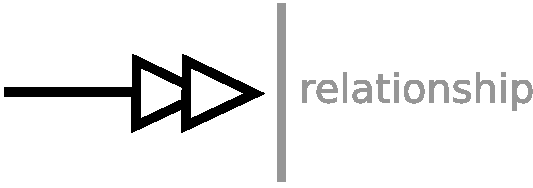
\includegraphics[scale = 0.5]{images/absoluteStimulation}
  \caption{The \ER glyph for \glyph{absolute stimulation}.}
  \label{fig:absoluteStimulation}
\end{figure}

%\normalcolor